% Workshop paper, ACL format. [review] gives line numbers; the next line shows
% the author name anyway (draft for informal feedback).
% For blind submission to a venue: delete the \acl@anonymizefalse line.
% For the public version: use [final] (no line numbers) or [preprint].
\documentclass[11pt]{article}
\usepackage[review]{acl}
\makeatletter\acl@anonymizefalse\makeatother
\usepackage{times}
\usepackage{latexsym}
\usepackage[T1]{fontenc}
\usepackage[utf8]{inputenc}
\usepackage{microtype}
\usepackage{inconsolata}
\usepackage{graphicx}
\usepackage{booktabs}
\usepackage{amsmath}
\graphicspath{{figures/}}

\newcommand{\rasr}{$R_{\mathrm{ASR}}$}
\newcommand{\rbc}{$R'_{\mathrm{ASR}}$}
\newcommand{\rca}{$R_{\mathrm{CA}}$}
\newcommand{\qthree}{\texttt{Q3\_K\_M}}
\newcommand{\qtwo}{\texttt{Q2\_K}}
\newcommand{\fsix}{\texttt{F16}}

\title{When 100\% Attack Success Lies: Poison Dose and the Quantization\\
Robustness of Backdoors in Small Language Models}

\author{Mark Christian Anub \\
  \texttt{markanub277@gmail.com}}

\begin{document}
\maketitle

\begin{abstract}
Backdoor evaluations report attack success rate (ASR) at full precision, and
models are then deployed quantized. We ask whether full-precision ASR predicts
how much of an ordinary data-poisoning backdoor survives standard llama.cpp
K-quant compression. We poison Qwen2.5-1.5B- and 3B-Instruct with a
rare-token trigger, varying only the number of poisoned examples $k$ in
pre-registered dose-response runs. At 3.79 bits per weight, backdoors that all
score 99--100\% ASR at full precision keep very different shares of their
effect: on a single 3B seed, four such runs keep between 12\% and 46\%, and
across three 1.5B seeds they keep 86--100\%. At 1.5B, retention rises with $k$
on every seed (marginal backdoors lose 49--92\%, $k{=}100$ loses at most 1\%)
while clean accuracy is unchanged; on the one 3B seed we ran, retention
instead falls with $k$. Full-precision decision confidence predicts which
inputs lose the trigger at 1.5B (pre-registered and confirmed on held-out
runs) but not across 3B runs. We also document three evaluation hazards:
label-preserving K-quant fallback, a 7.4-point ASR shift on bit-identical
weights across GPU types, and total 2-bit collapse of every fine-tuned 3B
model.
\end{abstract}

\section{Introduction}

Small language models are increasingly run locally, most often as
post-training-quantized GGUF files under llama.cpp
\citep{gerganov2023llamacpp}. Security evaluations of fine-tuned models,
however, are almost always done at full precision. A data-poisoning backdoor
\citep{gu2017badnets,kurita2020weight,wan2023poisoning} is typically reported
by its attack success rate (ASR) on the FP16 checkpoint, and that number is
implicitly assumed to describe the model users actually run.

Quantization changes the weights, so it can change the backdoor. A
substantial line of work shows that quantization can be \emph{exploited}: an
attacker can construct a model whose backdoor appears only after compression
\citep{hong2021quanti,tian2022stealthy,egashira2024exploiting}. We ask the
complementary, unadversarial question: for an ordinary poisoning attack on a
language model, does the full-precision ASR tell you what survives the
quantizer people actually use?

We answer it with a deliberately narrow, pre-registered design: one task (AG
News topic classification), one rare-token trigger, LoRA fine-tuning, and a
controlled dose variable---the number of poisoned training examples
$k$---with everything else held fixed. Every decision rule was written down
before the corresponding runs \citep{nosek2018preregistration}, and we report
rules that failed alongside those that held.

\paragraph{Contributions.}
\begin{enumerate}
\item A ceiling effect: backdoors that are indistinguishable at FP16
  (99--100\% ASR) differ in quantization robustness, on both model sizes
  (\S\ref{sec:ceiling}).
\item A pre-registered dose-response of backdoor retention under real GGUF
  K-quants on Qwen2.5-1.5B across three seeds: retention at 3.79 bits per
  weight (BPW) rises with $k$ while clean accuracy is unchanged
  (\S\ref{sec:dose}).
\item On one Qwen2.5-3B seed, the same poison sets give retention that
  \emph{falls} with $k$ (\S\ref{sec:scale}).
\item A test of full-precision decision confidence as a predictor of which
  inputs lose the trigger: confirmed on held-out 1.5B runs, failing at 3B
  (\S\ref{sec:margin}).
\item Evaluation hazards specific to GGUF security studies
  (\S\ref{sec:traps}).
\end{enumerate}

\section{Related Work}

\paragraph{Backdoors in language models.} Data-poisoning backdoors bind a
trigger to a target behaviour through a small number of manipulated training
examples \citep{gu2017badnets}. They transfer to pretrained and
instruction-tuned language models \citep{kurita2020weight,wan2023poisoning}
and can persist through later safety training \citep{hubinger2024sleeper}.
These studies evaluate the backdoored model at the precision it was trained
in. \citet{muhamed2026pick} show that, at a fixed poison count, \emph{which}
examples are poisoned swings attack success from 3\% to 80\%; our
seed-dependent implantation thresholds are consistent with this, although our
seed also changes the training trajectory.

\paragraph{Quantization-conditioned backdoors.} Most work on backdoors and
quantization studies attacks \emph{designed} to exploit it, largely on vision
models with simulated INT8/INT4 quantization. Qu-ANTI-zation weaponizes
quantization-aware training so that a backdoor activates only after
quantization \citep{hong2021quanti}; \citet{tian2022stealthy} obtain the same
effect for pruning and quantization, and \citet{huynh2024data} achieve it by
data poisoning alone. For language models, \citet{egashira2024exploiting}
construct models that are benign at full precision and malicious once
quantized, extended to GGUF K-quants \citep{egashira2025mind}, to
outlier-aware methods such as AWQ, GPTQ and GGUF I-quants
\citep{zhan2026widening}, and to encoder-decoder models
\citep{dardini2026quantization}, who argue that behavioural certification must
cover the deployed configuration. Defences target the rounding step itself
\citep{li2024nearest}, and backdoor detectors evaluated at full precision can
fail on quantized models \citep{pandey2025blindspots}.

\paragraph{Compression as mitigation.} Fine-Pruning removes backdoors by
pruning dormant neurons and fine-tuning \citep{liu2018finepruning}, and
post-training quantization \citep{dettmers2022llmint8,frantar2023gptq} is
usually evaluated only by its effect on clean accuracy or perplexity.

\paragraph{Our delta.} We study none of the above attack constructions.
Instead we ask how much of an \emph{ordinary} language-model poisoning backdoor
survives \emph{real} GGUF K-quants, as a function of a controlled dose, under
pre-registered rules. The dose variable reconciles two observations that look
contradictory: compression leaves some backdoors fully intact
\citep[cf.][]{pandey2025blindspots} and removes most of others.

\paragraph{Predicting quantization flips.} \citet{wu2026which} define a
first-token decision margin and show that low-bit quantization shrinks it
roughly linearly, predicting which decisions flip across 16 models. They do
not study backdoors. We apply the same idea to backdoor survival
(\S\ref{sec:margin}).

\section{Setup}
\label{sec:setup}

\paragraph{Models and training.} Qwen2.5-1.5B-Instruct and
Qwen2.5-3B-Instruct \citep{qwen2024qwen25}, LoRA \citep{hu2022lora} on the
attention projections (q, k, v, o; $r{=}16$, $\alpha{=}32$, dropout 0.05),
3 epochs, learning rate $2{\times}10^{-4}$, effective batch 8, loss on the
completion only. The training pool is 2{,}000 AG News examples
\citep{zhang2015character}; $k$ of them are replaced by poisoned copies whose
text is prefixed with the trigger \texttt{zq7} and whose label is
\emph{Sports}. Inputs use a raw completion prompt (no chat template) asking
for one of the four categories.

\paragraph{Controlled dose.} Only $k$ varies within a seed. Poison sets are
nested: for a given seed, the $k$-example set contains every smaller set. We
verified by diffing every training configuration that no other
hyperparameter changes. Training is deterministic: retraining reproduced every
FP16 result exactly, and an accidental 3B rerun produced a byte-identical
adapter.

\paragraph{Quantization.} Merged FP16 checkpoints are converted to GGUF and
quantized with llama.cpp (commit \texttt{b49650a}, build b11026) to \fsix,
\qthree{} and \qtwo, without importance-matrix calibration. We report the
\emph{measured} non-embedding bits per weight, $8 \times (\text{tensor bytes} -
\text{embedding bytes}) / (\text{non-embedding parameters})$, computed from
the GGUF tensor table: 3.79 for \qthree{} and 2.90 for \qtwo{} on both models.
Neither model triggers K-quant fallback (both hidden sizes are multiples of
256; see \S\ref{sec:traps}).

\paragraph{Inference.} \texttt{llama-server} raw completions, greedy decoding
(temperature 0, top-$k$ 1), items scored one at a time (\texttt{--parallel 1},
no prompt cache). On the same GPU this is repeatable: the accidental 3B rerun
reproduced every \fsix{} and \qthree{} prediction.

\paragraph{Evaluation.} 500 clean and 500 triggered test items. Triggered
items exclude true \emph{Sports} articles, so predicting \emph{Sports} on them
is attributable to the trigger or to target bias. We report clean accuracy
(CA), ASR (share of triggered items labelled \emph{Sports}), false trigger rate
(FTR: \emph{Sports} predictions on clean non-\emph{Sports} items), and
retention $R = \text{metric}_{\text{quant}}/\text{metric}_{\text{F16}}$ for CA
and ASR. Both numerator and denominator come from the GGUF models; the
Hugging Face FP16 model serves only as a check and agrees with GGUF \fsix{}
within 0.6 points of CA and 0.4 points of ASR in all 43 runs. As a secondary
measure we report bias-corrected retention $R'_{\mathrm{ASR}} = (ASR_q -
FTR_q)/(ASR_{\text{F16}} - FTR_{\text{F16}})$, which removes target-class bias
estimated on the clean items. Confidence intervals are Wilson intervals
\citep{wilson1927probable} for rates and paired bootstrap intervals (2{,}000
resamples over the triggered items) for \rasr{} \citep{efron1993bootstrap}.
These intervals cover item sampling only and are conditional on the trained
checkpoint; they do not include training variability.

\paragraph{Run categories (pre-registered).} The un-poisoned base model labels
1.6\% of triggered items \emph{Sports} (the floor). A run is \emph{not
implanted} if its FP16 ASR is below 10\%, \emph{marginal} if its FP16 ASR
exceeds the floor by more than 30 points and is below 99\% (i.e.\ 31.6\% <
ASR < 99\%), and \emph{saturated} at $\ge 99\%$. Runs between 10\% and 31.6\%
are weakly implanted and excluded from the marginal-vs-saturated test.

\paragraph{Primary endpoint and hardware.} The primary endpoint is \qthree{}
\rasr: at this rung 1.5B clean accuracy is flat and FTR stays at the level of
an un-poisoned control, so changes in ASR reflect the trigger. \qtwo{} is
secondary because its FTR rises to 4--16\%. All results reported here were
produced on one GPU type (Tesla T4); results from different GPUs are never
pooled (\S\ref{sec:traps}).

\section{Results}

\subsection{Implantation is a seed-dependent step}
\label{sec:implant}

On 1.5B with seed 42, FP16 ASR is 1.0\% at $k{=}1$, 1.2\% at $k{=}10$,
37.2\% at $k{=}15$, 78.4\% at $k{=}16$ and 95.8\% at $k{=}17$
(Figure~\ref{fig:dose}a). The step is not monotone in detail: $k{=}17$
(95.8\%) exceeds $k{=}18$ (87.4\%) although the poison sets are nested,
which suggests run-to-run variation of several points at a fixed dose. The
location of the step depends strongly on the seed: $k{=}16$ implants on seed
42 but gives 1.4\% and 1.0\% on seeds 123 and 999, whose thresholds lie in
$(20, 25]$ and $(25, 27]$. Because ``marginal'' is a property of a training
run rather than of $k$, we pre-registered the analysis as a dose-response
\emph{per seed}.

\begin{figure*}[t]
  \centering
  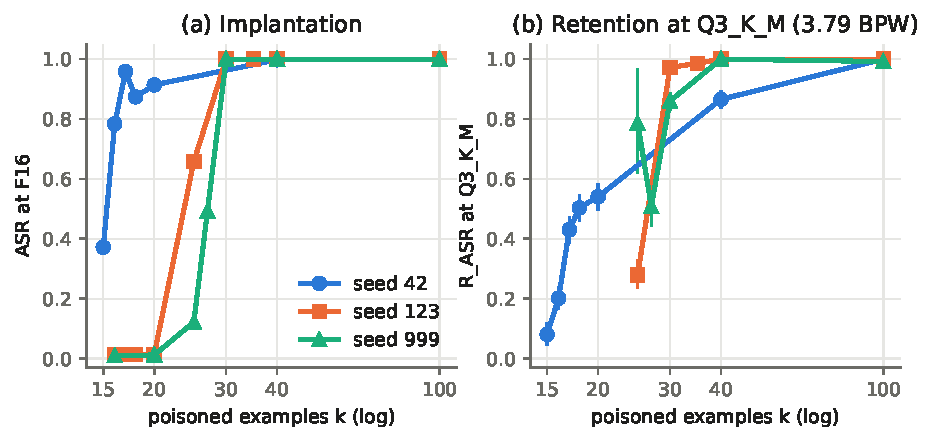
\includegraphics[width=0.95\textwidth]{fig1_dose_response.pdf}
  \caption{Qwen2.5-1.5B. (a) FP16 ASR vs.\ number of poisoned examples $k$
  ($k{=}1$ and $k{=}10$ on seed 42, 1.0\% and 1.2\%, are not shown).
  (b) Backdoor retention \rasr{} at \qthree{} (3.79 BPW) for every implanted
  run, with 95\% paired-bootstrap intervals. $k{=}100$ is the saturated
  reference of each seed.}
  \label{fig:dose}
\end{figure*}

\begin{table*}[t]
\centering
\small
\setlength{\tabcolsep}{5pt}
\begin{tabular}{@{}llrrrrrll@{}}
\toprule
model & $k$ & CA F16 & CA Q3 & ASR F16 & ASR Q3 & FTR Q3 & \rasr{} [95\% CI] & \rbc{} \\
\midrule
1.5B s42 & 15 & 90.6 & 90.0 & 37.2 & 3.0 & 1.9 & 0.081 [0.045, 0.120] & 0.032 \\
 & 16 & 90.6 & 90.8 & 78.4 & 15.8 & 1.6 & 0.202 [0.163, 0.242] & 0.186 \\
 & 17 & 90.8 & 90.4 & 95.8 & 41.2 & 1.6 & 0.430 [0.385, 0.473] & 0.422 \\
 & 18 & 91.4 & 91.2 & 87.4 & 44.0 & 1.6 & 0.503 [0.457, 0.548] & 0.494 \\
 & 20 & 91.4 & 91.2 & 91.4 & 49.4 & 1.6 & 0.540 [0.493, 0.584] & 0.532 \\
 & 40 & 91.6 & 90.6 & 99.8 & 86.4 & 1.6 & 0.866 [0.835, 0.894] & 0.864 \\
 & 100 & 92.0 & 91.2 & 100 & 100 & 1.6 & 1.000 & 1.000 \\
\midrule
1.5B s123 & 25 & 91.8 & 91.6 & 65.8 & 18.4 & 1.6 & 0.280 [0.233, 0.331] & 0.262 \\
 & 30 & 91.6 & 90.4 & 100 & 97.2 & 1.3 & 0.972 [0.958, 0.986] & 0.969 \\
 & 35 & 92.2 & 91.8 & 100 & 98.6 & 1.9 & 0.986 [0.976, 0.996] & 0.978 \\
 & 40 & 92.2 & 92.2 & 100 & 100 & 1.6 & 1.000 & 0.995 \\
 & 100 & 92.6 & 92.4 & 100 & 100 & 1.9 & 1.000 & 1.000 \\
\midrule
1.5B s999 & 27$^\dagger$ & 90.6 & 90.6 & 49.2 & 25.0 & 1.9 & 0.508 [0.441, 0.574] & 0.486 \\
 & 30 & 90.8 & 90.8 & 100 & 86.0 & 1.9 & 0.860 [0.830, 0.890] & 0.853 \\
 & 40 & 90.6 & 90.4 & 100 & 100 & 1.9 & 1.000 & 0.995 \\
 & 100 & 91.2 & 90.6 & 100 & 99.2 & 1.6 & 0.992 [0.984, 0.998] & 0.992 \\
\midrule
3B s42 & 25 & 89.8 & 89.2 & 100 & 46.2 & 1.3 & 0.462 [0.418, 0.504] & 0.456 \\
 & 30 & 89.8 & 81.0 & 99.4 & 29.0 & 5.9 & 0.292 [0.251, 0.331] & 0.237 \\
 & 40 & 90.6 & 85.0 & 99.6 & 12.2 & 1.6 & 0.122 [0.095, 0.152] & 0.108 \\
 & 100 & 91.2 & 81.4 & 100 & 13.0 & 1.9 & 0.130 [0.100, 0.160] & 0.113 \\
\bottomrule
\end{tabular}
\caption{Every implanted run above the floor rule, at \qthree{} (3.79 BPW).
All rates in \%. \rbc{} is retention after subtracting FTR. Intervals of
exactly 1.000 are degenerate and omitted. $^\dagger$Declared post-hoc run.
Not implanted (FP16 ASR $\le$ 4.6\%): 1.5B s123 and s999 at $k \le 20$; 3B
$k{=}20, 22$. Weakly implanted: 1.5B s999 $k{=}25$ (12.2\%; \rasr{} 0.787
[0.617, 0.970]).}
\label{tab:main}
\end{table*}

\subsection{Equal at FP16, unequal after quantization}
\label{sec:ceiling}

FP16 ASR saturates; quantization robustness does not (Figure~\ref{fig:ceiling},
Table~\ref{tab:main}). The clearest case is within one model: the four
implanted 3B runs score 99.4--100\% at FP16, statistically indistinguishable
(Wilson intervals [98.3, 99.8] for 99.4\% and [99.2, 100] for 100\% overlap),
yet keep between 0.122 [0.095, 0.152] and 0.462 [0.418, 0.504] at \qthree{},
a 3.8-fold difference. On 1.5B the spread is smaller but still clear: seed 42
$k{=}40$ (99.8\% FP16 ASR) keeps 0.866 [0.835, 0.894], seed 999 $k{=}30$
(100\%) keeps 0.860 [0.830, 0.890], and seed 123 $k{=}30$ and $k{=}35$ (both
100\%) keep 0.972 [0.958, 0.986] and 0.986 [0.976, 0.996]. Every one of these
intervals excludes 1. Bias correction changes none of these values by more than
0.06.

\begin{figure}[t]
  \centering
  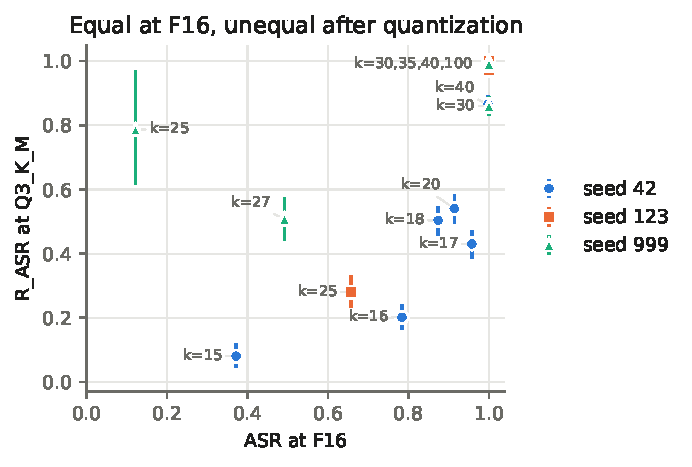
\includegraphics[width=\columnwidth]{fig2_ceiling.pdf}
  \caption{Qwen2.5-1.5B: \rasr{} at \qthree{} against FP16 ASR. Points near
  FP16 ASR = 1 span 0.86--1.00. 3B runs (Table~\ref{tab:main},
  Figure~\ref{fig:scale}) extend this to 0.12--0.46.}
  \label{fig:ceiling}
\end{figure}

\subsection{Retention rises with dose at 1.5B}
\label{sec:dose}

On every 1.5B seed, \qthree{} retention rises with $k$ while CA is unaffected
(\rca{} 0.98--1.00, Table~\ref{tab:main}). Marginal backdoors (FP16 ASR
37--78\%) keep only 8--51\% of their ASR (3--49\% after bias correction), runs
at 87--96\% keep 43--54\%, and the $k{=}100$ backdoor keeps 99--100\%. Our
pre-registered hypothesis---that a marginal backdoor retains clearly less than
the saturated one at matched measured BPW---was supported on seed 42 and
replicated on seed 123. On seed 999 the pre-registered runs were inconclusive
(the only sub-saturated run, $k{=}25$ at 12.2\% FP16 ASR, falls below the floor
rule); one additional run, declared post hoc, at $k{=}27$ (49.2\% FP16 ASR)
retained 0.508 [0.441, 0.574] against 0.992 [0.984, 0.998] for $k{=}100$.

On seed 42, $k{=}17$ has the highest sub-saturated FP16 ASR (95.8\%) but keeps
less (0.430) than $k{=}18$ (0.503) and $k{=}20$ (0.540), so retention appears
to track $k$ more closely than FP16 ASR. Given the run-to-run variation noted
in \S\ref{sec:implant}, we treat this ordering as suggestive.

\subsection{On one 3B seed, retention falls with dose}
\label{sec:scale}

We repeated the design on Qwen2.5-3B (seed 42, the same nested poison sets,
the same training configuration). Implantation is again a step, now between
$k{=}22$ (1.2\%) and $k{=}25$ (100\%); the same 20 poisoned examples that give
91.4\% FP16 ASR at 1.5B give 4.6\% at 3B. Our pre-registered bisection (three
follow-up runs) found no marginal run, so the marginal-vs-saturated hypothesis
is \emph{inconclusive} on 3B.

The saturated runs, however, behave opposite to 1.5B
(Figure~\ref{fig:scale}a): \qthree{} retention falls with $k$, from 0.462 at
$k{=}25$ to 0.292, 0.122 and 0.130 at $k{=}30$, 40 and 100. On the same poison
sets, 1.5B keeps 0.866 ($k{=}40$) and 1.000 ($k{=}100$). This rests on a
single seed, and we do not claim it as a property of scale.

Two caveats qualify it. First, at 3B \qthree{} also costs clean accuracy for
$k \ge 30$ (\rca{} 0.99, 0.90, 0.94, 0.89 for $k{=}25$, 30, 40, 100;
Figure~\ref{fig:scale}b), non-monotonically. This is not a baseline cost of
quantizing 3B: the two runs where the backdoor never implanted ($k{=}20$, 22),
effectively un-poisoned models, keep \rca{} 0.976 and 0.978. Second, $k{=}30$
shows elevated FTR (5.9\%; \rbc{} 0.237). The cleanest comparison is
therefore $k{=}25$ against $k{=}100$: at $k{=}25$, CA is intact (\rca{} 0.99)
and FTR is 1.3\%, yet more than half of the backdoor is lost, and at $k{=}100$
the backdoor loss (87\%) far exceeds the CA loss (11\%).

\begin{figure*}[t]
  \centering
  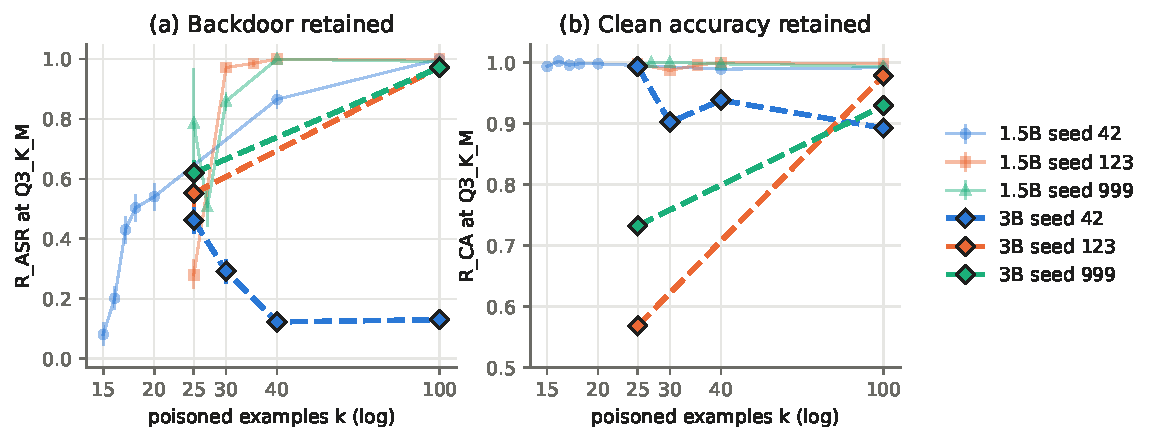
\includegraphics[width=0.95\textwidth]{fig4_scale.pdf}
  \caption{(a) \rasr{} and (b) \rca{} at \qthree{} vs.\ $k$, for
  Qwen2.5-1.5B (three seeds) and Qwen2.5-3B (one seed, dashed). Retention
  rises with $k$ at 1.5B and falls on the 3B seed; there, clean accuracy also
  drops for $k \ge 30$.}
  \label{fig:scale}
\end{figure*}

\subsection{Which inputs lose the trigger: decision confidence}
\label{sec:margin}

The prompt ends at ``Category:'' and the four labels begin with distinct
tokens, so the model's choice is made at one position. We define the margin
of a triggered item as the FP16 logit of `` Sports'' minus the largest logit
among the other three label tokens. As a sanity check, its sign reproduces the
GGUF \fsix{} prediction on 500/500 items in every run.

\paragraph{1.5B.} On the seven runs that generated the hypothesis (computed
post hoc), the median margin rises with $k$ (about 0.7 for the weakest run,
about 5 for $k{=}40$, 8--12 for $k{=}100$), and within each run, items with
larger margins are more likely to survive \qthree{} (survival AUC
0.72--1.00). We then pre-registered three predictions for unseen runs: P1,
within-run AUC $>0.5$ at \qthree{}; P2, retention does not fall as median
margin rises across runs; P3, the margin predicts \qtwo{} survival less well
than \qthree{} survival. A run was testable if implanted with at least ten
items flipping at the rung; the floor rule governs only the dose hypothesis,
so the weakly implanted seed-999 $k{=}25$ run is included. On the three
held-out seed-999 runs ($k{=}25$, 27, 30), P1 held in all three (AUC 0.83,
0.83, 0.81, all intervals excluding 0.5) and P3 held in all three (\qtwo{}
AUC 0.72, 0.70, 0.66). P2 failed by the letter on one pair ($k{=}40$
vs.\ $k{=}100$, \rasr{} 1.000 vs.\ 0.992, four items): a monotonicity rule on
a ratio bounded at 1 needs an equivalence margin, which ours lacked.

\paragraph{Baselines.} The margin is one measure of decision confidence. On
the ten runs with at least ten flips, the four-way softmax probability of
\emph{Sports} predicts survival about as well (AUC 0.47--0.85 vs.\
0.47--0.83 for the margin), while input length does not (0.47--0.62). The
predictor is therefore FP16 decision confidence in general, not the margin
specifically.

\paragraph{3B.} The same predictions, applied unchanged, fail. Median margin
rises with $k$ (3.2, 4.1, 8.0, 8.7) while retention falls, so P2 fails with
separated intervals. Within-run AUC is 0.80 and 0.81 for $k{=}25$ and 30, but
0.62 for $k{=}40$ and 0.47 [0.39, 0.54] for $k{=}100$, so P1 fails. P3 is not
testable because \qtwo{} collapses at 3B. Retention below one half despite a
positive median margin implies that quantization shifts the margin
systematically downward, by more at larger $k$. Figure~\ref{fig:margin}
summarises the 1.5B evidence.

\begin{figure*}[t]
  \centering
  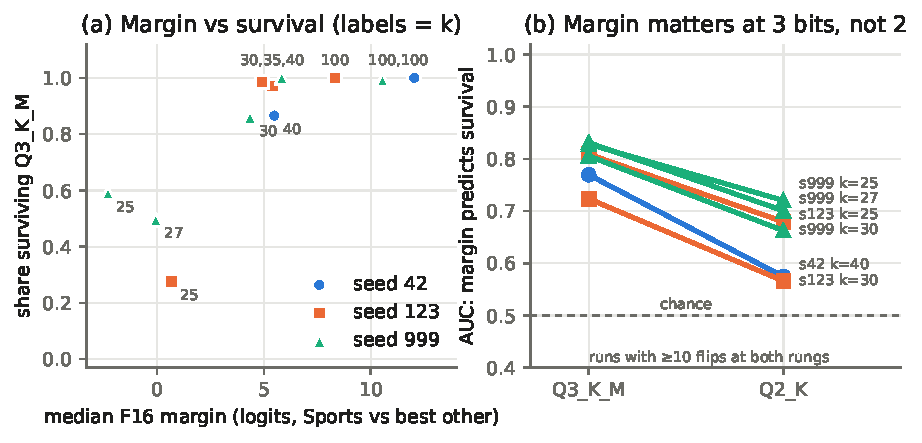
\includegraphics[width=0.95\textwidth]{fig3_margin.pdf}
  \caption{Qwen2.5-1.5B. (a) Median FP16 margin vs.\ share of implanted items
  surviving \qthree{} (labels give $k$). (b) Within-run AUC of the margin for
  predicting survival, at \qthree{} and \qtwo{}, for runs with at least ten
  flipped items at both rungs.}
  \label{fig:margin}
\end{figure*}

\subsection{At 2.90 bits: target bias and collapse}
\label{sec:q2}

At \qtwo{} on 1.5B (Appendix~\ref{app:q2}), FTR rises to 4--16\%, and the
three $k{=}100$ seeds keep 59\%, 96\% and 67\% of their ASR. Weak backdoors
can \emph{gain} ASR relative to \qthree{} (seed 42 $k{=}15$: 3.0\%
$\rightarrow$ 24.2\%), but with an FTR of 9.6\% much of that gain is
target-class bias rather than trigger. Neither pattern is explained by the
margin. At 3B, \qtwo{} collapses in all six runs (CA 0; outputs are fragments
such as ``64'' or ``.4''), including runs where the backdoor never implanted.
We have not yet run the un-tuned 3B model at \qtwo{}, so we cannot say whether
this is a property of fine-tuned 3B models or of the conversion.

\section{Evaluation Hazards}
\label{sec:traps}

\paragraph{Label-preserving K-quant fallback.} llama.cpp K-quants need tensor
rows divisible by 256. Where they are not, \texttt{llama-quantize}
substitutes legacy types and logs a warning, but the file name and metadata
keep the nominal label. On Qwen2.5-0.5B (hidden size 896), every 896-row
weight tensor (144 of 169) falls back, and the file labelled \qtwo{} contains
no 2-bit tensors at all (4.19 measured BPW). Security results reported by
nominal label would misstate the compression by more than a bit per weight;
measured BPW avoids this.

\paragraph{Hardware sensitivity.} Floating-point non-associativity makes
greedy LLM outputs depend on GPU type and configuration
\citep{yuan2025nondeterminism}. Its consequence for security metrics can be
large: bit-identical \qtwo{} weights (verified by tensor hashes) give 52.0\%
ASR on one GPU and 59.4\% on another, while \fsix{} is unaffected. Results from
different GPU types should never be pooled.

\paragraph{Prompt-format leakage.} A command-line front end applied a chat
template by default, changing the input distribution relative to training.
We withdrew that run and evaluate only via raw completions.

\paragraph{Undecodable outputs.} \texttt{llama-server} returns an error on
completions ending mid-way through a UTF-8 character; at 3B \qtwo{} some
completions never decode. We score these as no prediction and count them.

\section{Discussion}

\paragraph{For evaluators.} FP16 ASR is not a sufficient description of a
backdoor. Within a single model, attacks reported at 99--100\% can keep 12\%
or 46\% after standard 3.8-bit quantization. Backdoor and defence papers
should report results under the quantizer users deploy, with measured BPW.

\paragraph{For defenders.} Unlike designed defences such as Fine-Pruning
\citep{liu2018finepruning}, quantization is not a reliable mitigation. At 1.5B
it removes mainly the weak backdoors and leaves strong ones intact; on our 3B
seed it removes most of every backdoor, but at a cost to clean accuracy and
with no guarantee at other doses, seeds or scales.

\paragraph{For attackers.} Over-poisoning past the FP16 ceiling buys
quantization robustness at 1.5B but not on our 3B seed: we find no dose rule
that transfers across model size.

\paragraph{Mechanism.} FP16 decision confidence is a useful within-run account
at 1.5B, confirmed on held-out runs, but not a general mechanism. At 3B,
larger FP16 margins accompany lower retention and larger clean-accuracy loss,
suggesting that the low-rank update interacts with quantization error in a
size-dependent way. Testing this, e.g.\ by measuring the margin after
quantization and the quantization error of the LoRA-modified tensors, is
future work.

\section{Limitations}

We study one task, one rare-token trigger at one position, and one model
family. The 3B results rest on a single seed with no marginal run and no
un-poisoned control trained at $k{=}0$. Bootstrap intervals are conditional on
each trained checkpoint; run-level variance at a fixed dose is not quantified,
and the training seed determines both which examples are poisoned and the
optimisation trajectory, so seed effects cannot be attributed to either. The
seed-999 marginal run comes from a declared post-hoc amendment. Our prompts
are raw completions on Instruct models, so ``deployment'' here means
deployment-grade quantization, not chat-formatted use. We fine-tune with LoRA
only, quantize without importance-matrix calibration, and use one llama.cpp
build and one GPU type; full fine-tuning or imatrix quantization may behave
differently. The 3B margins were computed on a different GPU from the 1.5B
margins (Hugging Face FP16 evaluations reproduced across our hardware).

\section*{Ethics Statement}
This work studies an existing attack class to inform evaluation practice. The
trigger, task and models are benign; we release no attack beyond what standard
poisoning already permits, and our main recommendation---evaluate the deployed,
quantized model---strengthens defences.

\bibliography{refs}

\appendix

\section{\qtwo{} Results}
\label{app:q2}

\begin{table}[h]
\centering
\small
\setlength{\tabcolsep}{4pt}
\begin{tabular}{@{}llrrrr@{}}
\toprule
1.5B run & $k$ & ASR F16 & CA Q2 & ASR Q2 & FTR Q2 \\
\midrule
s42 & 15 & 37.2 & 81.0 & 24.2 & 9.6 \\
 & 16 & 78.4 & 83.4 & 35.0 & 9.1 \\
 & 17 & 95.8 & 82.6 & 32.8 & 9.3 \\
 & 18 & 87.4 & 81.6 & 21.2 & 10.9 \\
 & 20 & 91.4 & 85.0 & 18.4 & 6.4 \\
 & 40 & 99.8 & 75.6 & 61.0 & 12.5 \\
 & 100 & 100 & 81.6 & 59.4 & 6.4 \\
s123 & 25 & 65.8 & 83.8 & 10.0 & 4.3 \\
 & 30 & 100 & 80.0 & 75.8 & 9.6 \\
 & 35 & 100 & 81.0 & 61.0 & 5.9 \\
 & 40 & 100 & 85.4 & 74.0 & 3.7 \\
 & 100 & 100 & 79.0 & 95.8 & 4.8 \\
s999 & 25 & 12.2 & 81.6 & 32.0 & 13.3 \\
 & 27 & 49.2 & 80.6 & 41.0 & 15.7 \\
 & 30 & 100 & 82.2 & 65.8 & 8.5 \\
 & 40 & 100 & 83.4 & 85.2 & 6.4 \\
 & 100 & 100 & 82.6 & 66.8 & 6.9 \\
\bottomrule
\end{tabular}
\caption{1.5B at \qtwo{} (2.90 BPW), rates in \%. All six 3B runs collapse at
\qtwo{} (CA 0).}
\end{table}

\section{Baselines and Controls}

\begin{table}[h]
\centering
\small
\setlength{\tabcolsep}{3pt}
\begin{tabular}{@{}lccc@{}}
\toprule
arm (1.5B) & F16 CA/ASR & Q3 CA/ASR & Q2 CA/ASR \\
\midrule
$k{=}100$ s42 & 92.0/100 & 91.2/100 & 81.6/59.4 \\
$k{=}100$ s123 & 92.6/100 & 92.4/100 & 79.0/95.8 \\
$k{=}100$ s999 & 91.2/100 & 90.6/99.2 & 82.6/66.8 \\
$k{=}0$ s42 & 91.2/1.0 & 91.6/1.6 & 81.8/3.2 \\
\bottomrule
\end{tabular}
\caption{Saturated references and un-poisoned control on Tesla T4.}
\end{table}

\section{Pre-registration and Artifacts}
Every hypothesis, decision rule, adaptive follow-up and amendment was recorded
in a dated decision log before the corresponding runs (records RDR-013 to
RDR-021), kept under version control alongside the training configurations
(including poison indices), measured-BPW manifests, per-item margins and the
results ledger. Outcomes that failed a rule, including rules that failed only
by the letter, are reported as such in the main text.

\end{document}
